\scanpage{153}
% archive foliation: 152
3. \uline{Application à la caractérisation des \deleted{\unsure{revêtements}}\inserted{\unsure{variétés}} étales \unsure{locaux}} \deleted{\unsure{finis}} \margin{Cf plus bas.}

\figure{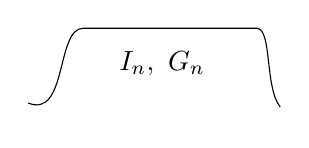
\begin{tikzpicture}[x=1cm,y=1cm]
\node at (1.7,0) {$I_n,\ G_n$};
\draw (0,-.5) .. controls (.5,-.7) and (.35,.45) .. (.7,.45) -- (2.9,.45) .. controls (3.1,.45) and (3,-.3) .. (3.2,-.55);
\end{tikzpicture}}

\uline{Prop 3.\unsure{2|1}.} Soit $f:X\to Y$ un morphisme fini, \unsure{($n$ un entier)}.

Conditions équivalentes

(i) $f$ est étale, et le rang de $X$ en un pt de $Y$ est partout égal à $n$.

(ii) Il existe un $Y_1\to Y$ fid plat tel que $X\times_Y Y_1$ soit $Y_1$-isomorphe à $Y_1\times I_n$.

(ii bis) Kif-kif, avec $Y_1$ \deleted{\unsure{étale}} rev. étale galoisien (de groupe $G_n$ si on veut)

(iii) $X$ est isomorphe à un $P/\deleted{\unsure{G}}H$, où $P$ est un rev. étale galoisien de $Y$, de groupe $G$, et $H$ un sous-groupe de $G$.

(iii bis) Kif kif, avec $G=G_n$, $H=G_{n-1}$ \inserted{(une \unsure{dimension})} (stabilisateur d'un pt de $I_n$).

\figure{\begin{tikzpicture}[x=1cm,y=1cm]
\draw (0,4.8) -- (.18,.3) .. controls (.2,0) and (.35,.05) .. (.5,-.1);
\draw (-.7,5.8) .. controls (-.5,4.8) and (-1,3.6) .. (-.95,2.8) .. controls (-1.2,2) and (-.6,2.2) .. (-.7,1.5) .. controls (-.9,.4) and (-.4,-.6) .. (-.3,-1);
\end{tikzpicture}}

\margin{$\unsure{(i)|(iii)}\Rightarrow\unsure{(iii\ \mathrm{bis})|(ii\ \mathrm{bis})}$ \unsure{théorème de Galois},
$\unsure{(iii)}\Rightarrow(ii\ \mathrm{bis})$ immédiat
car les \uline{propriétés} des \uline{\unsure{morphismes}} sont \uline{compatibles} avec \uline{images réciproques}.
$(ii)\Rightarrow(i)$ par la descente.}

\[
(i)\Longrightarrow(iii\ \mathrm{bis})
\]
(la démonstration \inserted{ainsi que le résultat} qui suit, due à \inserted{J.P.} Serre).
On fait opérer $G_n$ sur $X\times\cdots\times X$ ($n$ facteurs, produit sur $Y$), de façon évidente.
L'ensemble des pts d'isotropie est \deleted{fermé et ouvert}\inserted{réunion de composantes} connexes (car si $s\in G_n$ est dans le groupe d'isotropie d'un pt $x$, il opère trivialement sur
